Artificial neural networks (ANNs) play a crucial role in modern HEP analyses. The \VH{} analysis makes use of them extensively, with all signal regions employing classification ANNs, developed specifically to distinguish signal from background in their specific regions. Additionally, a regression neural network is deployed in the \wh{} analysis to estimate the \pt{} of the associated vector boson, which is needed for the STXS analysis. This chapter will provide a brief overview of neural networks.

\section{ANN Overview}
The simplest ANN structure is the feed-forward neural network (Figure~\ref{fig:ann_image}), which consists of several ``layers'' that apply linear transformations sequentially to an input vector, $\vec{x}$. Each layer applies a nonlinear ``activation'' function $\sigma(x)$ element-wise to the output of the linear transformation: 
\begin{equation}
  \sigma({[x_{1}, x_{2}, \ldots, x_{N}]}^{T}) = {[\sigma(x_{1}), \sigma(x_{2}), \ldots, \sigma(x_{N})]}^{T},
\end{equation}
where $N$ is the dimension of the input vector. Each layer is thus defined by a weight matrix (kernel), a bias vector, and an activation function. This can be written concisely as
\begin{equation}
  \vec{y} = \sigma(\textbf{W}\cdot\vec{x} + \vec{b}),
\end{equation}
where $\textbf{W}$ is the weight matrix, $\vec{b}$ is the bias vector, and $\vec{y}$ the resulting output vector. A single layer contains $N \times M + M$ trainable parameters, where $N$ and $M$ are the dimensions of the input and output vectors, respectively.

\begin{figure}[htp]
  \centering
  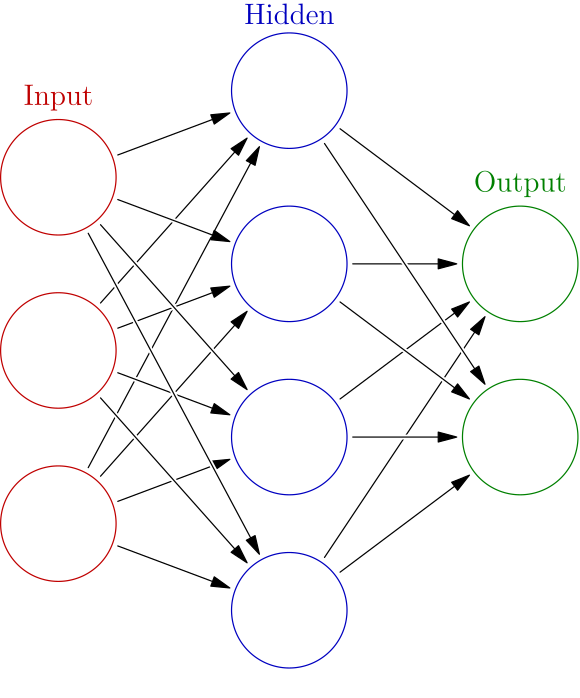
\includegraphics[width=0.4\textwidth]{figures/nn/nn_image.png}
  \caption{A simple feed-forward neural network. Each network starts with an input layer, can have any number of hidden layers, and ends with an output layer. Each circular node represents a neuron, with an arrow representing a connection from the output of one neuron to the input of another~\cite{ColoredNN}.}\label{fig:ann_image}
\end{figure}

Several commonly used activation functions include:
\begin{itemize}
  \item \texttt{ReLU} (Rectified Linear Unit): $\sigma(x) = \max(0, x)$
  \item \texttt{ELU} (Exponential Linear Unit): $\sigma(x) = x$ if $x > 0$, else $\sigma(x) = e^{x} - 1$
  \item \texttt{Sigmoid}: $\sigma(x) = \frac{1}{1 + e^{-x}}$
  \item \texttt{Swish}: $\sigma(x) = \frac{x}{1 + e^{-x}}$
  \item \texttt{Hyperbolic Tangent}: $\sigma(x) = \tanh(x)$
  \item \texttt{Softmax}: $\sigma(\vec{x})= \frac{e^{x_{i}}}{\sum_{i=1}^{N}e^{x_{i}}}$
\end{itemize}
Note that the softmax activation function is applied to the entire input vector and ensures the output elements sum to one.

In a classification ANN, the network is trained with input vectors paired with known truth labels, which aims to reproduce the correct truth labels at its output. The predicted labels, which are constrained between zero and one, can be interpreted as a probability that a given input belongs to a particular class. The training of the network consists of minimizing a ``loss'' function by adjusting the network's weights and biases, which quantifies the difference between the predicted outputs and the truth labels. 

The most widely used training method is backpropagation~\cite{backpropagation} which is a type of stochastic gradient descent (SGD) used to optimize the networks parameters. More advanced SGD variants, including Adam~\cite{kingma2017adammethodstochasticoptimization} and Nadam~\cite{dozat2016}, are now seeing widespread use.

Prior to training, it is standard practice to apply feature scaling to the input vectors. This ensures all features are of a similar numerical value, which helps prevent any one feature from dominating due to its magnitude, and allowing optimization algorithms to converge faster. Common scaling methods include: 
\begin{itemize}
  \item \texttt{StandardScaler}: Scales features to have a mean of zero and a variance of one.
  \item \texttt{RobustScaler}: Scales features using the median and interquartile range, making it robust to outliers.
  \item \texttt{MinMaxScaler}: Scales features to a specified range, typically between zero and one or negative one and one.
\end{itemize}
Training of the ANN is performed in batches, where each batch is a subset of the training data. The number of samples in each batch represents the batch size. The ANNs kernel and bias vectors are updated at the end of each batch. One cycle through the training data is known as an epoch. 

For binary classifiers, the most common loss function is the binary cross-entropy, defined as:
\begin{equation}
  \mathcal{L} = -\frac{1}{N}\sum_{i=1}^{N} \left( y_{i}\log(\hat{y}_{i}) + (1 - y_{i})\log(1 - \hat{y}_{i}) \right),
\end{equation}
where $y_{i}$ is the truth label, $\hat{y}_{i}$ is the predicted label, and $N$ the number of input vectors. For multi-class classification where an ANN has more than two output categories, the categorical cross-entropy is used, defined as:
\begin{equation}
  \mathcal{L} = -\frac{1}{N}\sum_{i=1}^{N} \sum_{j=1}^{M} y_{ij}\log(\hat{y}_{ij}),
\end{equation}
where $y_{ij}$ is the truth label for the $j$-th class of the $i$-th input vector, $\hat{y}_{ij}$ is the predicted label for the $j$-th class of the $i$-th input vector, and $M$ is the number of truth classes.

Neural networks can also be used for regression tasks, where the goal is to predict a continuous value rather than a class label. These are trained in a similar manner to classification networks, except the output layer typically does not contain an activation function, to ensure a continuous value at the output. Additionally, the loss function for classification networks is not suitable for regression networks, and instead there are several other loss functions used, consisting of:
\begin{itemize}
  \item \texttt{Mean Squared Error (MSE)}: $\mathcal{L} = \frac{1}{N}\sum_{i=1}^{N} (y_{i} - \hat{y}_{i})^{2}$
  \item \texttt{Mean Absolute Error (MAE)}: $\mathcal{L} = \frac{1}{N}\sum_{i=1}^{N} |y_{i} - \hat{y}_{i}|$
  \item \texttt{Huber Loss}: $\mathcal{L} = \frac{1}{N}\sum_{i=1}^{N}
  \begin{cases}
    \frac{1}{2}(y_{i} - \hat{y}_{i})^{2} & \text{if } |y_{i} - \hat{y}_{i}| < \delta \\
    \delta(|y_{i} - \hat{y}_{i}| - \frac{1}{2}\delta) & \text{otherwise}
  \end{cases}$
\end{itemize}

\section{ANN In The \VH{} Analysis}
The training in the \VH{} analysis includes four classification networks and one regression network, all implemented using \texttt{Keras}~\cite{chollet2015keras} with the \texttt{TensorFlow} (TF)~\cite{tensorflow2015-whitepaper} backend. To improve training performance, input features are normalized using the \texttt{StandardScaler} transformation. For the classification networks, class imbalances between signal and background samples are addressed by modifying event weights such that the average signal weight is normalized to one, and each background is scaled to have the same sum of weights as the signal. Additionally, each signal region uses two ANNs, one of which is trained on events with odd event numbers and the other with even event numbers. This is done to ensure that inference can be performed on events not used in the network training by using the odd-trained ANN with even events and vice versa. To prevent overfitting, early stopping is applied by monitoring the validation loss during training. If no improvement is observed for 50 consecutive epochs, training is stopped and the model is reverted to the weights corresponding to the lowest validation loss.

The hyperparameters, such as the number of layers, number of nodes per layer, and other tunable parameters, are optimized with \texttt{Keras-Tuner}~\cite{omalley2019kerastuner} with the Hyperband algorithm~\cite{li2018hyperband}. This algorithm is a successive halving algorithm that effectively explores hyperparameter space by training a large number of neural networks for a few epochs, and discarding the worst performant half, while the better performing ones are trained longer. This process repeats iteratively until the best performing model is selected.

The optimal hyperparameters are validated using a K-fold cross-validation technique to ensure they generalize well to unseen data. For the \wh{} analysis, a 5-fold cross-validation is used. If the model shows consistent performance across the folds, it is considered robust enough, and thus the final model is retrained, taking advantage of the full training dataset.

Finally, because the ANNs for each signal region are multi-classifiers, a single neural network discriminant must be constructed that combines the output nodes into one variable suitable for the statistical analysis. It was found that for both signal regions, the optimal discriminant is defined as:
\begin{equation}
  ANN_{\Delta} = \ln{\frac{ANN_{\wh}}{\sum_{B}ANN_{B}}},
\end{equation}
where the numerator corresponds to the probability of being a \wh{} event, and the denominator corresponds to the probability of being any of the trained upon backgrounds.

